% Copyright 2006 by Till Tantau
%
% This file may be distributed and/or modified
%
% 1. under the LaTeX Project Public License and/or
% 2. under the GNU Free Documentation License.
%
% See the file doc/generic/pgf/licenses/LICENSE for more details.

\section{Nodes and Edges}

\label{section-nodes}

\subsection{Overview}

In the present section, the usage of \emph{nodes} in
\tikzname\ is explained. A node is typically a rectangle or circle or
another simple shape with some text on it. 

Nodes are added to paths using the special path
operation |node|. Nodes \emph{are not part of the path
  itself}. Rather, they are added to the picture after the path has
been drawn. 

In Section~\ref{section-nodes-basic} the basic syntax of the node
operation is explained, followed in Section~\ref{section-nodes-multi}
by the syntax for multi-part nodes, which are nodes that contain
several different text parts. After this, the different options for
the text in nodes are explained. In
Section~\ref{section-nodes-anchors} the concept of \emph{anchors} is
introduced along with their usage. In
Section~\ref{section-nodes-transformations} the different ways
transformations affect nodes are
studied. Sections~\ref{section-nodes-placing-1}
and~\ref{section-nodes-placing-2} are about placing nodes on or next
to straight lines and curves. In
Section~\ref{section-nodes-connecting} it is explained how a node can
be used as a ``pseudo-coordinate.'' Section~\ref{section-nodes-edges}
introduces the |edge| operation, which
works similar to the |to| operation and also similar to the |node|
operation. Finally, Section~\ref{section-nodes-executing} explains the
special |after node path| options.


\subsection{Nodes and Their Shapes}

\label{section-nodes-basic}

In the simplest case, a node is just some text that is
placed at some coordinate. However, a node can also have a border
drawn around it or have a more complex background and
foreground. Indeed, some nodes do not have a text at all, but consist
solely of the background. You can name nodes so that you can reference
their coordinates later in the same picture or, if certain precautions
are taken as explained in Section~\ref{section-cross-picture-tikz},
also in different pictures.

There are no special \TeX\ commands for adding a node to a picture; rather,
there is path operation called |node| for this. Nodes are created
whenever \tikzname\ encounters |node| or |coordinate| at a point on a
path where it would expect a normal path operation (like |-- (1,1)| or
|sin (1,1)|). It is also possible to give node specifications
\emph{inside} certain path operations as explained later.

The node operation is typically followed by some options, which apply
only to the node. Then, you can optionally \emph{name} the node by
providing a name in round braces. Lastly, for the |node| operation you
must provide some label text for the node in curly braces, while for
the |coordinate| operation you may not. The node is placed at the
current position of the path \emph{after the path has been
  drawn}. Thus, all nodes are drawn ``on top'' of the path and
retained until the path is complete. If there are several nodes on a
path, they are drawn on top of the path in the order they are
encountered. 

\begin{codeexample}[]
\tikz \fill[fill=examplefill]
     (0,0) node {first node}
  -- (1,1) node {second node}
  -- (0,2) node {third node};
\end{codeexample}

The syntax for specifying nodes is the following:
\begin{pathoperation}{node}{\opt{|[|\meta{options}|]|}\opt{|(|\meta{name}|)|}%
    \opt{|at(|\meta{coordinate}|)|}\opt{\marg{text}}}
  The effect of |at| is to place the node at the coordinate given
  after |at| and not, as would normally be the case, at the last
  position. The |at| syntax is not available when a node is given
  inside a path operation (it would not make any sense, there).
  
  The |(|\meta{name}|)| is a name for later reference and it is
  optional. You may also add the option |name=|\meta{name} to the
  \meta{option} list; it has the same effect.

  \begin{key}{/tikz/name=\meta{node name}}
    Assigns a name to the node for later reference. Since this is a
    ``high-level'' name (drivers never know of it), you can use spaces,
    number, letters, or whatever you like when naming a node. Thus, you
    can name a node just |1| or perhaps |start of chart| or even
    |y_1|. Your node name should \emph{not} contain any punctuation like
    a dot, a comma, or a colon since these are used to detect what kind
    of coordinate you mean when you reference a node. 
  \end{key}

  \begin{key}{/tikz/at=\meta{coordinate}}
    This is another way of specifying ath |at| coordinate. Note that,
    typically, you will have to enclose the \meta{coordinate} in curly
    braces so that a comma inside the \meta{coordinate} does not
    confuse \TeX.
  \end{key}

  The \meta{options} is an optional list of options that \emph{apply
    only to the node} and have no effect outside. The other way round,
  most ``outside'' options also apply to the node, but not all. For
  example, the ``outside'' rotation does not apply to nodes (unless some
  special options are used, sigh). Also, the outside path action, like
  |draw| or |fill|, never applies to the node and must be given in the
  node (unless some special other options are used, deep sigh).

  As mentioned before, we can add a border and even a background to a
  node:  
\begin{codeexample}[]
\tikz \fill[fill=examplefill]
      (0,0) node {first node}
   -- (1,1) node[draw] {second node}
   -- (0,2) node[fill=red!20,draw,double,rounded corners] {third node};
\end{codeexample}

  The ``border'' is actually just a special case of a much more general
  mechanism. Each node has a certain \emph{shape} which, by default, is
  a rectangle. However, we can also ask \tikzname\ to use a circle shape
  instead or an ellipse shape (you have to include |pgflibraryshapes| for
  the latter shape): 

\begin{codeexample}[]
\tikz \fill[fill=examplefill]
      (0,0) node{first node}
   -- (1,1) node[ellipse,draw] {second node}
   -- (0,2) node[circle,fill=red!20] {third node};
\end{codeexample}

  In the future, there might be much more complicated shapes available
  such as, say, a shape for a resistor or a shape for a \textsc{uml}
  class. Unfortunately, creating new shapes is a bit tricky and makes
  it necessary to use the basic layer directly. Life is hard.

  To select the shape of a node, the following option is used:
  \begin{key}{/tikz/shape=\meta{shape name} (initially rectangle)}
    Select the shape either of the current node or, when this option is
    not given inside a node but somewhere outside, the shape of all
    nodes in the current scope.%
    \indexoption{\meta{shape name}}

    Since this option is used often, you can leave out the
    |shape=|. When \tikzname\ encounters an option like |circle|
    that it does not know, it will, after everything else has failed,
    check whether this option is the name of some shape. If so, that
    shape is selected as if you had said |shape=|\meta{shape name}.

    By default, the following shapes are available: |rectangle|,
    |circle|, |coordinate|, and, when the package |pgflibraryshapes| is
    loaded, also |ellipse|. Details of these shapes, like their anchors
    and size options, are discussed in Section~\ref{section-the-shapes}.
  \end{key}
  
  The following styles influences how nodes are rendered:
  \begin{stylekey}{/tikz/every node (initially \normalfont empty)}
    This style is installed at the beginning of every node. 
\begin{codeexample}[]
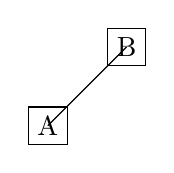
\begin{tikzpicture}[every node/.style={draw}]
  \draw (0,0) node {A} -- (1,1) node {B};
\end{tikzpicture}
\end{codeexample}
  \end{stylekey}
  \begin{stylekey}{/tikz/every \meta{shape} node (initially \normalfont empty)}
    These styles are installed at the beginning of a node of a given
    \meta{shape}. For example, |every rectangle node| is used for
    rectangle nodes, and so on.
\begin{codeexample}[]
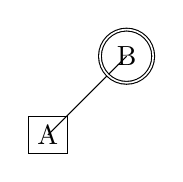
\begin{tikzpicture}
  [every rectangle node/.style={draw}, 
   every circle node/.style={draw,double}]
  \draw (0,0) node[rectangle] {A} -- (1,1) node[circle] {B};
\end{tikzpicture}
\end{codeexample}
  \end{stylekey}
\end{pathoperation}

There is a special syntax for specifying ``light-weighed'' nodes:

\begin{pathoperation}{coordinate}{\opt{|[|\meta{options}|]|}|(|\meta{name}|)|\opt{|at(|\meta{coordinate}|)|}}
  This has the same effect as

  |node[shape=coordinate][|\meta{options}|](|\meta{name}|)at(|\meta{coordinate}|){}|,
  
  where the |at| part might be missing.
\end{pathoperation}

Since nodes are often the only path operation on paths, there are two
special commands for creating paths containing only a node:

\begin{command}{\node}
  Inside |{tikzpicture}| this is an abbreviation for |\path node|.
\end{command}

\begin{command}{\coordinate}
  Inside |{tikzpicture}| this is an abbreviation for |\path coordinate|.
\end{command}


\subsubsection{Predefined Shapes}

\label{section-nodes-predefined}

\label{section-the-shapes}

\pgfname\ and \tikzname\ define three shapes, by default:
\begin{itemize}
\item
  |rectangle|,
\item
  |circle|, and
\item
  |coordinate|.
\end{itemize}
By loading library packages, you can define more shapes like ellipses
or diamonds; see Section~\ref{section-libs-shapes} for the complete
list of shapes. 

\label{section-tikz-coordinate-shape}
The |coordinate| shape is handled in a special way by \tikzname. When
a node |x| whose shape is |coordinate| is used as a coordinate |(x)|,
this has the same effect as if you had said |(x.center)|. None  of the
special ``line shortening rules'' apply in this case. This can be
useful since, normally, the line shortening causes paths to be
segmented and they cannot be used for filling. Here is an example that
demonstrates the difference: 
\begin{codeexample}[]
\begin{tikzpicture}[every node/.style={draw}]
  \path[yshift=1.5cm,shape=rectangle]
    (0,0) node(a1){} (1,0) node(a2){}
    (1,1) node(a3){} (0,1) node(a4){};
  \filldraw[fill=examplefill] (a1) -- (a2) -- (a3) -- (a4);
  
  \path[shape=coordinate]
    (0,0) coordinate(b1) (1,0) coordinate(b2)
    (1,1) coordinate(b3) (0,1) coordinate(b4);
  \filldraw[fill=examplefill] (b1) -- (b2) -- (b3) -- (b4);
\end{tikzpicture}
\end{codeexample}



\subsubsection{Common Options: Separations, Margins, Padding and
  Border Rotation}

\label{section-shape-seps}
\label{section-shape-common-options}

The exact behaviour of shapes differs, shapes defined for more
special purposes (like a, say, transistor shape) will have even more
custom behaviors. However, there are some options that apply to most
shapes:

\begin{key}{/pgf/inner sep=\meta{dimension} (initially .3333em)}
  \keyalias{tikz}
  An additional (invisible) separation space of \meta{dimension} will
  be added inside the shape, between the text and the shape's
  background path. The effect is as if you had added appropriate
  horizontal and vertical skips at the beginning and end of the text
  to make it a bit ``larger.''

  For those familiar with \textsc{css}, this is the same as
  \emph{padding}. 

\begin{codeexample}[]
\begin{tikzpicture}
  \draw (0,0)     node[inner sep=0pt,draw] {tight}
        (0cm,2em) node[inner sep=5pt,draw] {loose}
        (0cm,4em) node[fill=examplefill]   {default};
\end{tikzpicture}
\end{codeexample}
\end{key}

\begin{key}{/pgf/inner xsep=\meta{dimension} (initially .3333em)}
  \keyalias{tikz}
  Specifies the inner separation in the $x$-direction, only.
\end{key}

\begin{key}{/pgf/inner ysep=\meta{dimension} (initially .3333em)}
  \keyalias{tikz}
  Specifies the inner separation in the $y$-direction, only.
\end{key}  

\begin{key}{/pgf/outer sep=\meta{dimension} (initially .5\string\pgflinewidth)}
  \keyalias{tikz}
  This option adds an additional (invisible) separation space of
  \meta{dimension} outside the background path. The main effect of
  this option is that all anchors will move a little ``to the
  outside.''

  For those familiar with \textsc{css}, this is same as \emph{margin}.

  The default for this option is half the line width. When the default
  is used and when the background path is draw, the anchors will lie
  exactly on the ``outside border'' of the path (not on the path
  itself). When the shape is filled, but not drawn, this may not be
  desirable. In this case, the |outer sep| should be set to zero
  point. 
\begin{codeexample}[]
\begin{tikzpicture}
  \draw[line width=5pt]
    (0,0) node[outer sep=0pt,fill=examplefill]     (f) {filled}
    (2,0) node[inner sep=.5\pgflinewidth+2pt,draw] (d) {drawn};

  \draw[->] (1,-1) -- (f);
  \draw[->] (1,-1) -- (d);  
\end{tikzpicture}
\end{codeexample}
\end{key}

\begin{key}{/pgf/outer xsep=\meta{dimension} (initially .5\string\pgflinewidth)}
  \keyalias{tikz}
  Specifies the outer separation in the $x$-direction, only.
\end{key}

\begin{key}{/pgf/outer ysep=\meta{dimension} (initially .5\string\pgflinewidth)}
  \keyalias{tikz}
  Specifies the outer separation in the $y$-direction, only.
\end{key}

\begin{key}{/pgf/minimum height=\meta{dimension} (initially 0pt)}
  \keyalias{tikz}
  This option ensures that the height of the shape (including the
  inner, but ignoring the outer separation) will be at least
  \meta{dimension}. Thus, if the text plus the inner separation is not
  at least as large as \meta{dimension}, the shape will be enlarged 
  appropriately. However, if the text is already larger than
  \meta{dimension}, the shape will not be shrunk.
\begin{codeexample}[]
\begin{tikzpicture}
  \draw (0,0) node[minimum height=1cm,draw] {1cm}
        (2,0) node[minimum height=0cm,draw] {0cm};
\end{tikzpicture}
\end{codeexample}
\end{key}

\begin{key}{/pgf/minimum width=\meta{dimension} (initially 0pt)}
  \keyalias{tikz}
  Same as |minimum height|, only for the width.
\begin{codeexample}[]
\begin{tikzpicture}
  \draw (0,0) node[minimum height=2cm,minimum width=3cm,draw] {$3 \times 2$};
\end{tikzpicture}
\end{codeexample}
\end{key}

\begin{key}{/pgf/minimum size=\meta{dimension}}
  \keyalias{tikz}
  Sets both the minimum height and width at the same time.
\begin{codeexample}[]
\begin{tikzpicture}
  \draw (0,0)  node[minimum size=2cm,draw] {square};
  \draw (0,-2) node[minimum size=2cm,draw,circle] {circle};
\end{tikzpicture}
\end{codeexample}
\end{key}

\begin{key}{/pgf/shape aspect=\meta{aspect ratio}}
  \keyalias{tikz}
  Sets a desired aspect ratio for the shape. For the |diamond| shape,
  this option sets the ratio between width and height of the shape.
\begin{codeexample}[]
\begin{tikzpicture}
  \draw (0,0)  node[shape aspect=1,diamond,draw] {aspect 1};
  \draw (0,-2) node[shape aspect=2,diamond,draw] {aspect 2};
\end{tikzpicture}
\end{codeexample}
\end{key}

\label{section-rotating-shape-borders}

Some shapes (but not all), support a special kind of rotation. This 
rotation affects only the border of a shape and is independent of the 
node contents, but \emph{in addition} to any other transformations.
	
\begin{codeexample}[]
\tikzstyle{every node}=[dart, shape border uses incircle, 
  inner sep=1pt, draw]
\begin{tikzpicture}
  \foreach \a/\b/\c in {A/0/0, B/45/0, C/0/45, D/45/45}
    \node [shape border rotate=\b, rotate=\c] at (\b/36,-\c/36) {\a};
\end{tikzpicture}
\end{codeexample}

There are two types of rotation: restricted and unrestricted. Which 
type of rotation is applied is determined by on how the shape border 
is constructed. If the shape border is contructed using an incircle, 
that is, a circle that tightly fits the node contents (including 
the |inner sep|), then the rotation can be unrestricted. If, however,
the border is constructed using the natural dimensions of the node
contents, the rotation is restricted to integer multiples of 90 
degrees.

Why should there be two kinds of rotation and border construction?
Borders constructed using the natural dimensions of the node contents
provide a much tighter fit to the node contents, but to maintain 
this tight fit, the border rotation must be restricted to integer 
multiples of 90 degrees. By using an incircle, unrestricted rotation
is possible, but the border will not make a very tight fit to the
node contents. 
	
\begin{codeexample}[]
\tikzstyle{every node}=[isosceles triangle, draw]
\begin{tikzpicture}
  \node {abc};
  \node [shape border uses incircle] at (2,0) {abc};
\end{tikzpicture}
\end{codeexample}

There are \pgfname{} keys determine how a shape border is 
contructed, and to specify its rotation.
It should be noted that not all shapes support these keys, so 
reference should be made to the documentation for individual 
shapes. 
	
\begin{key}{/pgf/shape border uses incircle=\opt{\meta{boolean}}
    (default true)}
  \keyalias{tikz}
  Determines if the border of a shape is constructed using the 
  incircle. If no value is given \meta{boolean} will take the default
  value |true|.
\end{key}


\begin{key}{/pgf/shape border rotate=\meta{angle} (initially 0)}
  \keyalias{tikz}
  Rotates the border of a shape independently of the node contents,
  but in addition to any other transformations. If the shape 
  border is not constructed using the incircle, the rotation will be
  rounded to the nearest integer multiple of 90 degrees when the
  shape is drawn. 
\end{key}

Note that if the border of the shape is rotated, 
the compass point anchors, and `text box' anchors (including 
|mid east|, |base west|, and so on), \emph{do not rotate}, but the 
other anchors do:
	
\begin{codeexample}[]
\tikzstyle{every node}=[shape=trapezium, draw, shape border uses incircle]
\begin{tikzpicture}
  \node at (0,0)  (A) {A};
  \node [shape border rotate=30] at (1.5,0) (B) {B};
  \foreach \s/\t in 
    {left side/base east, bottom side/north, bottom left corner/base}{
       \fill[red]  (A.\s) circle(1.5pt) (B.\s) circle(1.5pt);
       \fill[blue] (A.\t) circle(1.5pt) (B.\t) circle(1.5pt);
  }
\end{tikzpicture}
\end{codeexample}

Finally, a somewhat unfortunate side-effect of rotating shape borders 
is that the supporting shapes do not distinguish between 
|outer xsep| and |outer ysep|, and typically, the larger of the 
two values will be used. 




\subsection{Multi-Part Nodes}

\label{section-nodes-multi}

Most nodes just have a single simple text label. However, nodes of a
more complicated shapes might be made up from several \emph{node
  parts}. For example, in automata theory a so-called Moore state has
a state name, drawn in the upper part of the state circle, and an
output text, drawn in the lower part of the state circle. These two
parts are quite independent. Similarly, a \textsc{uml} class shape
would have a name part, a method part, and an attributes
part. Different molecule shape might use parts for the different atoms
to be drawn at the different positions, and so on.

Both \pgfname\ and \tikzname\ support such multipart nodes. On the
lower level, \pgfname\ provides a system for specifying that a shape
consists of several parts. On the \tikzname\ level, you specify the
different node parts by using the following command:

\begin{command}{\nodepart\marg{part name}}
  This command can only be used inside the \meta{text} argument of a
  |node| path operation. It works a little bit like a |\part| command
  in \LaTeX. It will stop the typesetting of whatever node part was
  typeset until now and then start putting all following text into the
  node part named \meta{part name}---until another |\partname| is
  encountered or until the node \meta{text} ends.

\begin{codeexample}[]
\begin{tikzpicture}
  \node [circle split,draw,double,fill=red!20]
  {
    % No \nodepart has been used, yet. So, the following is put in the
    % ``text'' node part by default.
    $q_1$ 
    \nodepart{lower} % Ok, end ``text'' part, start ``output'' part
    $00$
  }; % output part ended.
\end{tikzpicture}
\end{codeexample}

  You will have to lookup which parts are defined by a shape.

  The following styles influences node parts:
  \begin{stylekey}{/tikz/every \meta{part name} node part (initially
      \normalfont empty)}
    This style is installed at the beginning of every node part named
    \meta{part name}. 
\begin{codeexample}[]
\tikz [every lower node part/.style={red}]
  \node [circle split,draw] {$q_1$ \nodepart{lower} $00$};
\end{codeexample}
  \end{stylekey}
\end{command}



\subsection{Options for the Text in  Nodes}

\label{section-nodes-options}

The simplest option for the text in nodes is its color. Normally, this
color is just the last color installed using |color=|, possibly
inherited from another scope. However, it is possible to specificly
set the color used for text using the following option:

\begin{key}{/tikz/text=\meta{color}}
  Sets the color to be used for text labels. A |color=| option
  will immediately override this option.
\begin{codeexample}[]
\begin{tikzpicture}
  \draw[red]       (0,0) -- +(1,1) node[above]     {red};
  \draw[text=red]  (1,0) -- +(1,1) node[above]     {red};
  \draw            (2,0) -- +(1,1) node[above,red] {red};
\end{tikzpicture}
\end{codeexample}
\end{key}

Just like the color itself, you may also wish to set the opacity of
the text only. For this, use the option |text opacity| option, which
is detailed in Section~\ref{section-tikz-transparency}.

Next, you may wish to adjust the font used for the text. Use the
following option for this:
\begin{key}{/tikz/font=\meta{font commands}}
  Sets the font used for text labels. 
\begin{codeexample}[]
\begin{tikzpicture}
  \draw[font=\itshape] (1,0) -- +(1,1) node[above] {italic};
\end{tikzpicture}
\end{codeexample}
  A perhaps more useful example is the following:

\begin{codeexample}[]
\tikz [every text node part/.style={font=\itshape}, 
       every lower node part/.style={font=\footnotesize}]
  \node [circle split,draw] {state \nodepart{lower} output};
\end{codeexample}
\end{key}


Normally, when a node is typeset, all the text you give in the braces
is but in one long line (in an |\hbox|, to be precise) and the node
will become as wide as necessary.

You can change this behaviour using the following options. They allow
you to limit the width of a node (naturally, at the expense of its
height).

\begin{key}{/tikz/text width=\meta{dimension}}
  This option will put the text of a node in a box of the given width
  (more precisely, in a |{minipage}| of this width; for plain \TeX\ a
  rudimentary ``minipage emulation'' is used).

  If the node text is not as wide as \meta{dimension}, it will
  nevertheless be put in a box of this width. If it is larger, line
  breaking will be done.

  By default, when this option is given, a ragged right border will be
  used. This is sensible since, typically, these boxes are narrow and
  justifying the text looks ugly.
\begin{codeexample}[]
\tikz \draw (0,0) node[fill=examplefill,text width=3cm]
  {This is a demonstration text for showing how line breaking works.};  
\end{codeexample}
\end{key}

\begin{key}{/tikz/text justified}
  Causes the text to be justified instead of (right)ragged. Use this
  only with pretty broad nodes.
{%
\hbadness=10000
\begin{codeexample}[]
\tikz \draw (0,0) node[fill=examplefill,text width=3cm,text justified]
  {This is a demonstration text for showing how line breaking works.};  
\end{codeexample}
}
  In the above example, \TeX\ complains (rightfully) about three very
  badly typeset lines. (For this manual I asked \TeX\ to stop
  complaining by using |\hbadness=10000|, but this is a foul deed,
  indeed.) 
\end{key}

\begin{key}{/tikz/text ragged}
  Causes the text to be typeset with a ragged right. This uses the
  original plain \TeX\ definition of a ragged right border, in which
  \TeX\ will try to balance the right border as well as possible. This
  is the default.
\begin{codeexample}[]
\tikz \draw (0,0) node[fill=examplefill,text width=3cm,text ragged]
  {This is a demonstration text for showing how line breaking works.};  
\end{codeexample}
\end{key}

\begin{key}{/tikz/text badly ragged}
  Causes the right border to be ragged in the \LaTeX-style, in which
  no balancing occurs. This looks ugly, but it may be useful for very
  narrow boxes and when you wish to avoid hyphenations.
\begin{codeexample}[]
\tikz \draw (0,0) node[fill=examplefill,text width=3cm,text badly ragged]
  {This is a demonstration text for showing how line breaking works.};  
\end{codeexample}
\end{key}

\begin{key}{/tikz/text centered}
  Centers the text, but tries to balance the lines.
\begin{codeexample}[]
\tikz \draw (0,0) node[fill=examplefill,text width=3cm,text centered]
  {This is a demonstration text for showing how line breaking works.};  
\end{codeexample}
\end{key}

\begin{key}{/tikz/text badly centered}
  Centers the text, without balancing the lines.
\begin{codeexample}[]
\tikz \draw (0,0) node[fill=examplefill,text width=3cm,text badly centered]
  {This is a demonstration text for showing how line breaking works.};  
\end{codeexample}
\end{key}

In addition to changing the width of nodes, you can also change the
height of nodes. This can be done in two ways: First, you can use the
option |minimum height|, which ensures that the height of the whole
node is at least the given height (this option is described in more
detail later). Second, you can use the option |text height|, which
sets the height of the text itself, more precisely, of the \TeX\ text
box of the text. Note that the |text height| typically is not the
height of the shape's box: In addition to the |text height|, an
internal |inner sep| is added as extra space and the text depth is
also taken into account.

I recommend using |minimum size| instead of |text height| except for
special situations.

\begin{key}{/tikz/text height=\meta{dimension}}
  Sets the height of the text boxes in shapes. Thus, when you write
  something like |node {text}|, the |text| is first typeset, resulting
  in some box of a certain height. This height is then replaced by the
  height |text height|. The resulting box is then used to determine
  the size of the shape, which will typically be larger. When you
  write |text height=| without specifying anything, the ``natural''
  size of the text box remains unchanged.
\begin{codeexample}[]
\tikz \node[draw]                  {y};    
\tikz \node[draw,text height=10pt] {y};       
\end{codeexample}
\end{key}

\begin{key}{/tikz/text depth=\meta{dimension}}
  This option works like |text height|, only for the depth of the text
  box. This option is mostly useful when you need to ensure a uniform
  depth of text boxes that need to be aligned. 
\end{key}




\subsection{Placing Nodes}

\label{section-nodes-anchors}

When you place a node at some coordinate, the node is centered on this
coordinate by default. This is often undesirable and it would be
better to have the node to the right or above the actual coordinate.


\subsubsection{Placing Nodes Using Anchors}

\pgfname\ uses a so-called anchoring mechanism to give you a very fine
control over the placement. The idea is simple: Imaging a node of
rectangular shape of a certain size. \pgfname\ defines numerous anchor
positions in the shape. For example to upper right corner is called,
well, not ``upper right anchor,'' but the |north east| anchor of the
shape. The center of the shape has an anchor called |center| on top of
it, and so on. Here are some examples (a complete list is given in
Section~\ref{section-the-shapes}).

\medskip\noindent
\begin{tikzpicture}
  \path node[minimum height=2cm,minimum width=5cm,fill=blue!25](x) {Big node};
  \fill (x.north)      circle (2pt) node[above] {|north|}
        (x.north east) circle (2pt) node[above] {|north east|}
        (x.north west) circle (2pt) node[above] {|north west|}
        (x.west) circle (2pt)       node[left]  {|west|}
        (x.east) circle (2pt)       node[right] {|east|}
        (x.base) circle (2pt)       node[below] {|base|};
\end{tikzpicture}

Now, when you place a node at a certain coordinate, you can ask \tikzname\
to place the node shifted around in such a way that a certain
anchor is at the coordinate. In the following example, we ask \tikzname\
to shift the first node such that its  |north east| anchor is at
coordinate |(0,0)| and that the |west| anchor of the second node is at
coordinate |(1,1)|.

\begin{codeexample}[]
\tikz \draw           (0,0) node[anchor=north east] {first node}
            rectangle (1,1) node[anchor=west] {second node};
\end{codeexample}

Since the default anchor is |center|, the default behaviour is to
shift the node in such a way that it is centered on the current
position.

\begin{key}{/tikz/anchor=\meta{anchor name}}
  Causes the node to be shifted such that it's anchor \meta{anchor
  name} lies on the current coordinate.

  The only anchor that is present in all shapes is |center|. However,
  most shapes will at least define anchors in all ``compass
  directions.'' Furthermore, the standard shapes also define a |base|
  anchor, as well as |base west| and |base east|, for placing things on
  the baseline of the text.
  
  The standard shapes also define a |mid| anchor (and |mid west| and
  |mid east|). This anchor is half the height of the character ``x''
  above the base line. This anchor is useful for vertically centering
  multiple nodes that have different heights and depth. Here is an
  example:
\begin{codeexample}[]
\begin{tikzpicture}[scale=3,transform shape]
  % First, center alignment -> wobbles
  \draw[anchor=center] (0,1)  node{x} -- (0.5,1)  node{y} -- (1,1)  node{t};
  % Second, base alignment -> no wobble, but too high
  \draw[anchor=base]   (0,.5) node{x} -- (0.5,.5) node{y} -- (1,.5) node{t};
  % Third, mid alignment
  \draw[anchor=mid]    (0,0)  node{x} -- (0.5,0)  node{y} -- (1,0)  node{t};
\end{tikzpicture}
\end{codeexample}
\end{key}



\subsubsection{Simplified Placement Options}

Unfortunately, while perfectly logical, it is often rather
counter-intuitive that in order to place a node \emph{above} a given
point, you need to specify the |south| anchor. For this reason, there
are some useful options that allow you to select the standard anchors
more intuitively:

\begin{key}{/tikz/above=\meta{offset} (default 0pt)}
  Does the same as |anchor=south|. If the \meta{offset} is specified,
  the node is additionally shifted upwards by the given
  \meta{offset}. 
\begin{codeexample}[]
\tikz \fill (0,0) circle (2pt) node[above] {above};
\end{codeexample}
\begin{codeexample}[]
\tikz \fill (0,0) circle (2pt) node[above=2pt] {above};
\end{codeexample}
\end{key}

\begin{key}{/tikz/below=\meta{offset} (default 0pt)}
  Similar to |above|.
\end{key}

\begin{key}{/tikz/left=\meta{offset} (default 0pt)}
  Similar to |above|.
\end{key}

\begin{key}{/tikz/right=\meta{offset} (default 0pt)}
  Similar to |above|.
\end{key}

\begin{key}{/tikz/above left}
  Does the same as |anchor=south east|. Note that giving both |above|
  and |left| options does not have the same effect as |above left|,
  rather only the last |left| ``wins.'' Actually, this option also
  takes an \meta{offset} parameter, but using this parameter without
  using the |placements| library is deprecated. (The |placements|
  library changes the meaning of this parameter to something more
  sensible.) 
\begin{codeexample}[]
\tikz \fill (0,0) circle (2pt) node[above left] {above left};
\end{codeexample}
\end{key}

\begin{key}{/tikz/above right}
  Similar to  |above left|.
\begin{codeexample}[]
\tikz \fill (0,0) circle (2pt) node[above right] {above right};
\end{codeexample}
\end{key}

\begin{key}{/tikz/below left}
  Similar to |above left|.
\end{key}
\begin{key}{/tikz/below right}
  Similar to |above left|.
\end{key}

% A second set of options behaves similarly, namely the |above of|,
% |below of|, and so on options. They cause the same anchors to be set
% as the options without |of|, however, their parameter is different:
% You must provide the name of another node. The current node will then
% be placed, say, above this specified node at a distance given by the
% option |node distance|. 
% \begin{key}{/tikz/above of=\meta{node}}
%   This option causes the node to be placed at the distance
%   |node distance| above of \meta{node}. The anchor is |center|.
% \begin{codeexample}[]
% \begin{tikzpicture}[node distance=1cm]
%   \draw[help lines] (0,0) grid (3,2);
%   \node (a)                    {a};
%   \node (b) [above of=a]       {b};
%   \node (c) [above of=b]       {c};
%   \node (d) [right of=c]       {d};
%   \node (e) [below right of=d] {e};
% \end{tikzpicture}
% \end{codeexample}
% \end{key}

% \begin{key}{/tikz/above left of=\meta{node}}
%   Works like |above of|, only the node is now put above and left. The
%   |node distance| is the Euclidean distance between the two nodes, not
%   the $L_1$-distance.
% \end{key}

% \begin{key}{/tikz/above right of=\meta{node}}
%   Works similarly.
% \end{key}
% \begin{key}{/tikz/left of=\meta{node}}
%   Works similarly.
% \end{key}
% \begin{key}{/tikz/right of=\meta{node}}
%   Works similarly.
% \end{key}
% \begin{key}{/tikz/below of=\meta{node}}
%   Works similarly.
% \end{key}
% \begin{key}{/tikz/below left of=\meta{node}}
%   Works similarly.
% \end{key}
% \begin{key}{/tikz/below right of=\meta{node}}
%   Works similarly.
% \end{key}
% \begin{key}{/tikz/node distance=\meta{dimension}}
%   Sets the distance between nodes that are placed using the
%   |... of| options. Note that this distance is the distance between
%   the centers of the nodes, not the distance between their borders. 
% \end{key}



\subsubsection{Enhanced Placement Options}

While the standard placement options suffice for simple cases, the
|placements| library offers more convenient placement options.

\begin{tikzlibrary}{placements}
  The library defines additional options for placing nodes
  conveniently. It also redefines the standard options like |above| so
  that they give you better control of node placement.
\end{tikzlibrary}

When this library is loaded, the options like |above| behave
differently: 

Still missing...

\subsubsection{Chains}

Chains provide a convenient way of creating sequences of nodes that
are placed ``in a row.''

Still missing...


\subsection{Fitting Nodes to a Set of Coordinates}

\label{section-nodes-fitting}

It is sometimes desirable that the size and position of a node is not
given using anchors and size parameters, rather one would sometimes
have a box be placed and be sized such that it ``is just large enough
to contain this, that, and that point.'' This situation typically
arises when a picture has been drawn an, afterwards, parts of the
picture are supposed to be encircled or hilighted.

In this situation the |fit| option from the |fit| library is useful,
see Section~\ref{section-library-fit} for a the details. The idea is
that you may give the |fit| option to a node. The |fit| option expects
a list of coordinates (one after the other without commas) as its
parameter. The effect will be that the node's text area has exactly
the necessary size so that it contains all the given coordinates. Here
is an example:

\begin{codeexample}[]
\begin{tikzpicture}[level distance=8mm]
  \node (root) {root}
    child { node (a) {a} }
    child { node (b) {b}
      child { node (d) {d} }
      child { node (e) {e} } }
    child { node (c) {c} };

  \node[draw=red,thick,ellipse,fit=(root) (b) (d) (e)] {};
  \node[draw=blue,thick,ellipse,fit=(b) (c) (e)] {};
\end{tikzpicture}
\end{codeexample}

If you want to fill the fitted node you will usually have to place it
on a background layer.

\begin{codeexample}[]
\begin{tikzpicture}[level distance=8mm]
  \node (root) {root}
    child { node (a) {a} }
    child { node (b) {b}
      child { node (d) {d} }
      child { node (e) {e} } }
    child { node (c) {c} };

  \begin{pgfonlayer}{background}
    \node[fill=red!20,ellipse,fit=(root) (b) (d) (e)] {};
    \node[fill=blue!20,ellipse,fit=(b) (c) (e)] {};
  \end{pgfonlayer}
\end{tikzpicture}
\end{codeexample}

\subsection{Transformations}

\label{section-nodes-transformations}


It is possible to transform nodes, but, by default, transformations do
not apply to nodes. The reason is that you usually do \emph{not} want
your text to be scaled or rotated even if the main graphic is
transformed. Scaling text is evil, rotating slightly less so.

However, sometimes you \emph{do} wish to transform a node, for
example, it certainly sometimes makes sense to rotate a node by
90 degrees. There are two ways in which you can achieve this:

\begin{enumerate}
\item
  You can use the following option:
  \begin{key}{/tikz/transform shape}
    Causes the current ``external'' transformation matrix to be
    applied to the shape. For example, if you said
    |\tikz[scale=3]| and then say |node[transform shape] {X}|, you
    will get a ``huge'' X in your graphic.
  \end{key}
\item
  You can give transformation option \emph{inside} the option list of
  the node. \emph{These} transformations always apply to the node.
\begin{codeexample}[]
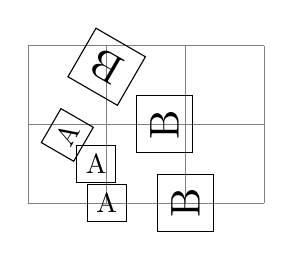
\begin{tikzpicture}[every node/.style={draw}]    
  \draw[help lines](0,0) grid (3,2);
  \draw            (1,0) node{A}
                   (2,0) node[rotate=90,scale=1.5] {B};
  \draw[rotate=30] (1,0) node{A}
                   (2,0) node[rotate=90,scale=1.5] {B};
  \draw[rotate=60] (1,0) node[transform shape] {A}
                   (2,0) node[transform shape,rotate=90,scale=1.5] {B};
\end{tikzpicture}
\end{codeexample}
\end{enumerate}




\subsection{Placing Nodes on a Line or Curve Explicitly}

\label{section-nodes-placing-1}

Until now, we always placed node on a coordinate that is mentioned in
the path. Often, however, we wish to place nodes on ``the middle'' of
a line and we do not wish to compute these coordinates ``by hand.''
To facilitate such placements, \tikzname\ allows you to specify that a
certain node should be somewhere ``on'' a line. There are two ways of
specifying this: Either explicitly by using the |pos| option or
implicitly by placing the node ``inside'' a path operation. These two
ways are described in the following.

\label{section-pos-option}

\begin{key}{/tikz/pos=\meta{fraction}}
  When this option is given, the node is not anchored on the last
  coordinate. Rather, it is anchored on some point on the line from
  the previous coordinate to the current point. The \meta{fraction}
  dictates how ``far'' on the line the point should be. A
  \meta{fraction} or 0 is the previous coordinate, 1 is the current
  one, everything else is in between. In particular, 0.5 is the
  middle.  

  Now, what is ``the previous line''? This depends on the previous
  path construction operation.

  In the simplest case, the previous path operation was a ``line-to''
  operation, that is, a  |--|\meta{coordinate} operation:
\begin{codeexample}[]
\tikz \draw (0,0) -- (3,1)
    node[pos=0]{0} node[pos=0.5]{1/2} node[pos=0.9]{9/10};
\end{codeexample}

  The next case is the curve-to operation (the |..| operation). In this
  case, the ``middle'' of the curve, that is, the position |0.5| is
  not necessarily the point at the exact half distance on the
  line. Rather, it is some point at ``time'' 0.5 of a point traveling
  from the start of the curve, where it is at time 0, to the end of
  the curve, which it reaches at time 0.5. The ``speed'' of the point
  depends on the length of the support vectors (the vectors that
  connect the start and end points to the control points). The exact
  math is a bit complicated (depending on your point of view, of
  course); you may wish to consult a good book on computer graphics
  and B�zier curves if you are intrigued. 
\begin{codeexample}[]
  \tikz \draw (0,0) .. controls +(right:3.5cm) and +(right:3.5cm) .. (0,3)
    \foreach \p in {0,0.125,...,1} {node[pos=\p]{\p}};
\end{codeexample}

  Another interesting case are the horizontal/vertical line-to operations
  \verb!|-! and \verb!-|!. For them, the position (or time) |0.5| is
  exactly the corner point.

\begin{codeexample}[]
\tikz \draw (0,0) |- (3,1)
  node[pos=0]{0} node[pos=0.5]{1/2} node[pos=0.9]{9/10};
\end{codeexample}

\begin{codeexample}[]
\tikz \draw (0,0) -| (3,1)
  node[pos=0]{0} node[pos=0.5]{1/2} node[pos=0.9]{9/10};
\end{codeexample}

  For all other path construction operations, \emph{the position
  placement does not work}, currently. This will hopefully change in
  the future (especially for the arc operation).  
\end{key}

\begin{key}{/tikz/auto=\meta{left or right} (default \normalfont is scope's setting)}
  This option causes an anchor positions to be calculated
  automatically according to the following rule. Consider a line
  between to points. If the \meta{direction} is |left|, then the
  anchor is chosen such that the node is to the left of this line. If
  the \meta{direction} is |right|, then the node is to the right of
  this line. Leaving out \meta{direction} causes automatic placement
  to be enabled with the last value of |left| or |right| used. A
  \meta{direction} of |false| disables automatic placement. This
  happens also  whenever an anchor is given explicitly by the
  |anchor| option or by one of the |above|, |below|, etc.\ options.

  This option only has an effect for nodes that are placed on lines or
  curves. 

\begin{codeexample}[]
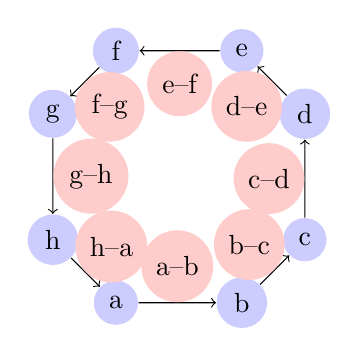
\begin{tikzpicture}
  [scale=.8,auto=left,every node/.style={circle,fill=blue!20}]
  \node (a) at (-1,-2) {a};
  \node (b) at ( 1,-2) {b};
  \node (c) at ( 2,-1) {c};
  \node (d) at ( 2, 1) {d};
  \node (e) at ( 1, 2) {e};
  \node (f) at (-1, 2) {f};
  \node (g) at (-2, 1) {g};
  \node (h) at (-2,-1) {h};

  \foreach \from/\to in {a/b,b/c,c/d,d/e,e/f,f/g,g/h,h/a}
    \draw [->] (\from) -- (\to)
               node[midway,fill=red!20] {\from--\to};
\end{tikzpicture}
\end{codeexample}
\end{key}

\begin{key}{/tikz/swap}
  This option exchanges the roles of |left| and |right| in automatic
  placement. That is, if |left| is the current |auto| placement,
  |right| is set instead and the other way round.
\begin{codeexample}[]
\begin{tikzpicture}[auto]
  \draw[help lines,use as bounding box] (0,-.5) grid (4,5);  

  \draw (0.5,0) .. controls (9,6) and (-5,6) .. (3.5,0)
    \foreach \pos in {0,0.1,0.2,0.3,0.4,0.5,0.6,0.7,0.8,0.9,1}
      {node [pos=\pos,swap,fill=red!20] {\pos}}
    \foreach \pos in {0.025,0.2,0.4,0.6,0.8,0.975}
      {node [pos=\pos,fill=blue!20] {\pos}};
\end{tikzpicture}
\end{codeexample}
\begin{codeexample}[]
\begin{tikzpicture}[shorten >=1pt,node distance=2cm,auto]
  \draw[help lines] (0,0) grid (3,2);

  \node[state] (q_0)                      {$q_0$};
  \node[state] (q_1) [above right of=q_0] {$q_1$};
  \node[state] (q_2) [below right of=q_0] {$q_2$};
  \node[state] (q_3) [below right of=q_1] {$q_3$};

  \path[->] (q_0) edge              node        {0} (q_1)
                  edge              node [swap] {1} (q_2)
            (q_1) edge              node        {1} (q_3)
                  edge [loop above] node        {0} ()
            (q_2) edge              node [swap] {0} (q_3)
                  edge [loop below] node        {1} ();
\end{tikzpicture}
\end{codeexample}
\end{key}

\begin{key}{/tikz/sloped}
  This option causes the node to be rotated such that a horizontal
  line becomes a tangent to the curve. The rotation is normally 
  done in such a way that text is never ``upside down.'' To get
  upside-down text, use can use |[rotate=180]| or
  |[allow upside down]|, see below.
\begin{codeexample}[]
\tikz \draw (0,0) .. controls +(up:2cm) and +(left:2cm) .. (1,3)
    \foreach \p in {0,0.25,...,1} {node[sloped,above,pos=\p]{\p}};
\end{codeexample}
\begin{codeexample}[]
\begin{tikzpicture}[->]
  \draw (0,0)   -- (2,0.5) node[midway,sloped,above] {$x$};
  \draw (2,-.5) -- (0,0)   node[midway,sloped,below] {$y$};
\end{tikzpicture}
\end{codeexample}
\end{key}


\begin{key}{/tikz/allow upside down=\meta{boolean} (default true, initially false)}
  If set to |true|, \tikzname\ will not ``righten'' upside down text. 
\begin{codeexample}[]
\tikz [allow upside down]
  \draw (0,0) .. controls +(up:2cm) and +(left:2cm) .. (1,3)
    \foreach \p in {0,0.25,...,1} {node[sloped,above,pos=\p]{\p}};
\end{codeexample}
\begin{codeexample}[]
\begin{tikzpicture}[->,allow upside down]
  \draw (0,0)   -- (2,0.5) node[midway,sloped,above] {$x$};
  \draw (2,-.5) -- (0,0)   node[midway,sloped,below] {$y$};
\end{tikzpicture}
\end{codeexample}
\end{key}


There exist styles for specifying positions a bit less ``technically'':
\begin{stylekey}{/tikz/midway}
  This has the same effect as |pos=0.5|.
\begin{codeexample}[]
\tikz \draw (0,0) .. controls +(up:2cm) and +(left:3cm) .. (1,5)
       node[at end]          {|at end|}
       node[very near end]   {|very near end|}
       node[near end]        {|near end|}
       node[midway]          {|midway|}
       node[near start]      {|near start|}
       node[very near start] {|very near start|}
       node[at start]        {|at start|};
\end{codeexample}
\end{stylekey}

\begin{stylekey}{/tikz/near start}
  Set to |pos=0.25|.
\end{stylekey}

\begin{stylekey}{/tikz/near end}
  Set to |pos=0.75|.
\end{stylekey}

\begin{stylekey}{/tikz/very near start}
  Set to |pos=0.125|.
\end{stylekey}

\begin{stylekey}{/tikz/very near end}
  Set to |pos=0.875|.
\end{stylekey}

\begin{stylekey}{/tikz/at start}
  Set to |pos=0|.
\end{stylekey}

\begin{stylekey}{/tikz/at end}
  Set to |pos=1|.
\end{stylekey}


\subsection{Placing Nodes on a Line or Curve Implicitly}

\label{section-nodes-placing-2}

When you wish to place a node on the line |(0,0) -- (1,1)|,
it is natural to specify the node not following the |(1,1)|, but
``somewhere in the middle.'' This is, indeed, possible and you can
write |(0,0) -- node{a} (1,1)| to place a node midway between |(0,0)| and
|(1,1)|.

What happens is the following: The syntax of the line-to path
operation is actually |--|
\opt{|node|\meta{node specification}}\meta{coordinate}. (It is even
possible to give multiple nodes in this way.) When the optional
|node| is encountered, that is, 
when the |--| is directly followed by |node|, then the
specification(s) are read and ``stored away.'' Then, after the
\meta{coordinate} has finally been reached, they are inserted again,
but with the |pos| option set.

There are two things to note about this: When a node specification is
``stored,'' its catcodes become fixed. This means that you cannot use
overly complicated verbatim text in them. If you really need, say, a
verbatim text, you will have to put it in a normal node following the
coordinate and add the |pos| option.

Second, which |pos| is chosen for the node? The position is inherited
from the surrounding scope. However, this holds only for nodes
specified in this implicit way. Thus, if you add the option
|[near end]| to a scope, this does not mean that \emph{all} nodes given
in this scope will be put on near the end of lines. Only the nodes
for which an implicit |pos| is added will be placed near the
end. Typically, this is what you want. Here are some examples that
should make this clearer:

\begin{codeexample}[]
\begin{tikzpicture}[near end]
  \draw (0cm,4em) -- (3cm,4em) node{A};    
  \draw (0cm,3em) --           node{B}          (3cm,3em);
  \draw (0cm,2em) --           node[midway] {C} (3cm,2em);
  \draw (0cm,1em) -- (3cm,1em) node[midway] {D} ;
\end{tikzpicture}
\end{codeexample}

Like the line-to operation, the curve-to operation |..| also allows you to
specify nodes ``inside'' the operation. After both the first |..| and
also after the second |..| you can place node specifications. Like for
the |--| operation, these will be collected and then reinserted after
the operation with the |pos| option set.


\subsection{The Label and Pin Options}

In addition to the |node| path operation, nodes can also be added
using the |label| and the |pin| option. This is mostly useful
for simple nodes. 

\begin{key}{/tikz/label=\opt{|[|\meta{options}|]|}\meta{angle}|:|\meta{text}}
  When this option is given to a |node| operation, it causes
  \emph{another} node to be added to the path after the current node
  has been finished. This extra node will have the text
  \meta{text}. It is placed according to the following rule: Suppose
  the |node| currently under construction is called |main node| and let us
  call the label node |label node|. Then the anchor of |label node| is
  placed at |main node.|\meta{angle}. The anchor that is chosen
  depends on the \meta{angle}. If the \meta{angle} lies between
  $-3^\circ$ and $+3^\circ$, then the anchor |west| is chosen, which
  causes |label node| to be placed right of the right end
  |main node|. If \meta{angle} lies between $4^\circ$ and $86^\circ$,
  the anchor |south west| is chosen, causing the |label node| to be
  placed above and right of the |main node|; and so on.
\begin{codeexample}[]
\tikz
  \node [circle,draw,label=60:$60^\circ$,label=below:$-90^\circ$] {my circle};
\end{codeexample}

  As can be seen in the above example, instead of specifying
  \meta{angle} as a number, it is also possible to use |left|,
  |right|, |above|, |above left|, and so on.

  You can pass \meta{options} to the node |label node|. For this, you
  provide the options in square brackets before the \meta{angle}. If you
  do so, you need to add braces around the whole argument of the
  |label| option and this is also the case if you have brackets or
  commas or semicolons or anything special in the \meta{text}.
\begin{codeexample}[]
\tikz \node [circle,draw,label={[red]above:X}] {my circle};
\end{codeexample}

\begin{codeexample}[]
\begin{tikzpicture}
  \node [circle,draw,label={[name=label node]above left:$a,b$}] {};
  \draw (label node) -- +(1,1);
\end{tikzpicture}
\end{codeexample}

  If you provide multiple |label| options, then multiple extra label
  nodes are added in the order they are given.

  The following styles influence how labels are drawn:
  \begin{key}{/tikz/label distance=\meta{distance} (initially 0pt)}
    The \meta{distance} is additionally inserted between the main node
    and the label node.
\begin{codeexample}[]
\tikz[label distance=5mm]
  \node [circle,draw,label=right:X,
                     label=above right:Y,
                     label=above:Z]       {my circle};
\end{codeexample}
  \end{key}
  \begin{stylekey}{/tikz/every label (initially \normalfont empty)}
    This style is used in every node created by the |label|
    option. The default is |draw=none,fill=none|.
  \end{stylekey}
\end{key}

\begin{key}{/tikz/pin=\opt{|[|\meta{options}|]|}\meta{angle}|:|\meta{text}}
  This is option is quite similar to the |label| option, but there is
  one difference: In addition to adding a extra node to the picture, 
  it also adds an edge from this node to the main node. This causes
  the node to look like a pin that has been added to the main node: 
\begin{codeexample}[]
\tikz \node [circle,fill=blue!50,minimum size=1cm,pin=60:$q_0$] {};
\end{codeexample}

  The meaning of the \meta{options} and the \meta{angle} and the
  \meta{text} is exactly the same as for the |node| option. Only, the
  options and styles the influence the way pins look are different:
  \begin{key}{/tikz/pin distance=\meta{distance} (initially 3ex)}
    This \meta{distance} is used instead of the |label distance| for
    the distance between the main node and the label node.
\begin{codeexample}[]
\tikz[pin distance=1cm]
  \node [circle,draw,pin=right:X,
                     pin=above right:Y,
                     pin=above:Z]       {my circle};
\end{codeexample}
  \end{key}
  \begin{stylekey}{/tikz/every pin (initially \normalfont draw=none,fill=none)}
    This style is used in every node created by the |pin|
    option.
  \end{stylekey}
  \begin{stylekey}{/tikz/every pin edge (initially help lines)}
    This style is used in every edge created by the |pin| optins.
\begin{codeexample}[]
\tikz [pin distance=15mm,
       every pin edge/.style={<-,shorten <=1pt,decorate,
                              decoration={snake,pre length=4pt}}]
  \node [circle,draw,pin=right:X,
                     pin=above right:Y,
                     pin=above:Z]       {my circle};
\end{codeexample}
  \end{stylekey}

  \begin{key}{/tikz/pin edge=\meta{options} (initially \normalfont empty)}
    This option can be used to set the options that are to be used
    in the edge created by the |pin| option. 
\begin{codeexample}[]
\tikz[pin distance=10mm]
  \node [circle,draw,pin={[pin edge={blue,thick}]right:X},
                     pin=above:Z]       {my circle};
\end{codeexample}
\begin{codeexample}[]
\tikz [every pin edge/.style={},
       initial/.style={pin={[pin distance=5mm,
                             pin edge={<-,shorten <=1pt}]left:start}}]
  \node [circle,draw,initial] {my circle};
\end{codeexample}
  \end{key}
\end{key}


\subsection{Connecting Nodes: Using Nodes as Coordinates}

\label{section-nodes-connecting}

Once you have defined a node and given it a name, you can use this
name to reference it. This can be done in two ways, see also
Section~\ref{section-node-coordinates}. Suppose you have said
|\path(0,0) node(x) {Hello World!};| in order to define a node named |x|. 
\begin{enumerate}
\item
  Once the node |x| has been defined, you can use
  |(x.|\meta{anchor}|)| wherever you would normally use a normal
  coordinate. This will yield the position at which the given
  \meta{anchor} is in the picture. Note that transformations do not
  apply to this coordinate, that is, |(x.north)| will be the northern
  anchor of |x| even if you have said |scale=3| or |xshift=4cm|. This
  is usually what you would expect.
\item
  You can also just use |(x)| as a coordinate. In most cases, this
  gives the same coordinate as |(x.center)|. Indeed, if the |shape| of
  |x| is |coordinate|, then |(x)| and |(x.center)| have exactly the
  same effect.

  However, for most other shapes, some path construction operations like
  |--| try to be ``clever'' when this they are asked to draw a line
  from such a coordinate or to such a coordinate. When you say
  |(x)--(1,1)|, the |--| path operation will not draw a line from the center
  of |x|, but \emph{from the border} of |x| in the direction going
  towards |(1,1)|. Likewise, |(1,1)--(x)| will also have the line
  end on the border in the direction coming from |(1,1)|.

  In addition to |--|, the curve-to path operation |..| and the path
  operations \verb!-|! and \verb!|-! will also handle nodes without
  anchors correctly. Here is an example, see also
  Section~\ref{section-node-coordinates}:
\begin{codeexample}[]
\begin{tikzpicture}
  \path (0,0) node             (x) {Hello World!}
        (3,1) node[circle,draw](y) {$\int_1^2 x \mathrm d x$};

  \draw[->,blue]   (x) -- (y);
  \draw[->,red]    (x) -| node[near start,below] {label} (y);
  \draw[->,orange] (x) .. controls +(up:1cm) and +(left:1cm) .. node[above,sloped] {label} (y);
\end{tikzpicture}
\end{codeexample}
\end{enumerate}




\subsection{Connecting Nodes: Using the Edge Operation}

\label{section-nodes-edges}

The |edge| operation works like a |to| operation that is added after
the main path has been drawn, much like a node is added after the main
path has been drawn. This allows you to have each |edge| to have a
different appearance. As the |node| operation, an |edge| temporarily
suspends the construction of the current path and a new path $p$ is 
constructed. This new path $p$ will be drawn after the main path has
been drawn. Note that $p$ can be totally different from the main
path with respect to its options. Also note that if there are
several |to| and/or |node| operations in the main path, each
creates its own path(s) and they are drawn in the order that they
are encountered on the path.

\begin{pathoperation}{edge}{\opt{|[|\meta{options}|]|}
    \opt{\meta{nodes}} |(|\meta{coordinate}|)|}
  The effect of the |edge| operation is that after the main path the
  following path is added to the picture:
  \begin{quote}
    |\path[every edge,|\meta{options}|] (\tikztostart) |\meta{path}|;|
  \end{quote}
  Here, \meta{path} is the |to path|. Note that, unlike the path added
  by the |to| operation, the |(\tikztostart)| is added before the
  \meta{path} (which is unnecessary for the |to| operation, since this
  coordinate is already part of the main path).

  The |\tikztostart| is the last coordinate on the path just before
  the |edge| operation, just as for the |node| or |to| operations. 
  However, there is one exception to this rule: If the |edge|
  operation is directly preceded by a |node| operation, then this
  just-declared node is the start coordinate (and not, as would
  normally be the case, the coordinate where this just-declared node
  is placed -- a small, but subtle difference). In this regard, |edge|
  differs from both |node| and |to|.
  
  If there are several |edge| operations in a row, the start coordinate
  is the same for all of them as their target coordiantes are not,
  after all, part of the main path. The start coordinate is, thus, the
  coordinate preceding the first |edge| operation. This is
  similar to nodes insofar as the |edge| operation does not modify the
  current path at all. In particular, it does not change the last
  coordinate visited, see the following example:
  
\begin{codeexample}[]
\begin{tikzpicture}
  \node (a) at   (0:1) {$a$};
  \node (b) at  (90:1) {$b$} edge [->]     (a);
  \node (c) at (180:1) {$c$} edge [->]     (a)
                             edge [<-]     (b);
  \node (d) at (270:1) {$d$} edge [->]     (a)
                             edge [dotted] (b)
                             edge [<-]     (c);  
\end{tikzpicture}
\end{codeexample}

  A different way of specifying the above graph using the |edge|
  operation is the following:  

\begin{codeexample}[]
\begin{tikzpicture}
  \foreach \name/\angle in {a/0,b/90,c/180,d/270}
    \node (\name) at (\angle:1) {$\name$};

  \path[->] (b) edge (a)
                edge (c)
                edge [-,dotted] (d)
            (c) edge (a)
                edge (d)
            (d) edge (a);
\end{tikzpicture}
\end{codeexample}

  As can be seen, the path of the |edge| operation inherits the
  options from the main path, but you can locally overrule them.

\begin{codeexample}[]
\begin{tikzpicture}
  \foreach \name/\angle in {a/0,b/90,c/180,d/270}
    \node (\name) at (\angle:1.5) {$\name$};

  \path[->] (b) edge            node[above right]  {$5$}     (a)
                edge                                         (c)
                edge [-,dotted] node[below,sloped] {missing} (d)
            (c) edge                                         (a)
                edge                                         (d)
            (d) edge [red]      node[above,sloped] {very}  
                                node[below,sloped] {bad}     (a);
\end{tikzpicture}
\end{codeexample}

  Instead of |every to|, the style |every edge| is installed at the
  beginning of the main path.
  \begin{stylekey}{/tikz/every edge (inititially draw)}
    Executed for each |edge|.
\begin{codeexample}[]
\begin{tikzpicture}[every to/.style={draw,dashed}]
  \path (0,0) to (3,2);
\end{tikzpicture}
\end{codeexample}
  \end{stylekey}
\end{pathoperation}


\subsection{Referencing Nodes Outside the Current Pictures}

\label{section-cross-picture-tikz}

\subsubsection{Referencing a Node in a Different Picture}

It is possible (but not quite trivial) to reference nodes in pictures
other than the current one. This means that you can create a picture
and a node therein and, later, you can draw a line from some other
position to this node. 

To reference nodes in different pictures, proceed as follows:
\begin{enumerate}
\item You need to add the |remember picture| option to all pictures
  that contain nodes that you wish to reference and also to all
  pictures from which you wish to reference a node in another
  picture.
\item You need to add the |overlay| option to paths or to whole
  pictures that contain references to nodes in different
  pictures. (This option switches the computation of the
  bounding box off.)
\item You need to use a driver that supports picture remembering and
  you need to run \TeX\ twice.
\end{enumerate}
(For more details on what is going on behind the scenes, see
Section~\ref{section-cross-pictures-pgf}.)

Let us have a look at the effect of these options.
\begin{key}{/tikz/remember picture=\meta{boolean} (initially false)}
  This option tells \tikzname\ that it should attempt to remember the
  position of the current picture on the page. This attempt may fail
  depending on which backend driver is used. Also, even if remembering
  works, the position may only be available on a second run of \TeX.

  Provided that remebering works, you may consider saying
\begin{codeexample}[code only]
\tikzsytle{every picture}+=[remember picture]
\end{codeexample}
  to make \tikzname\ remember all pictures. This will add one line in
  the |.aux| file for each picture in your document -- which typically
  is not very much. Then, you do not have to worry about remembered
  pictures at all.
\end{key}

\begin{key}{/tikz/overlay}
  This option is mainly intended for use when nodes in other pictures
  are referenced, but you can also use it in other situations. The
  effect of this option is that everything within the current scope is
  not taken into consideration when the bounding box of the current
  picture is computed.

  You need to specify this option on all paths (or at least on all
  parts of paths) that contain a reference to a node in another
  picture. The reason is that, otherwise, \tikzname\ will attempt to
  make the current picture large enough to encompass \emph{the node in
    the other picture}. However, on a second run of \TeX\ this will
  create an even bigger picture, leading to larger and larger
  pictures. Unless you know what you are doing, I suggest specifying
  the |overlay| option with all pictures that contain references to
  other pictures.
\end{key}

Let us now have a look at a few examples. These examples work only if
this document is processed with a driver that supports picture
remembering.
\medskip

\noindent\begin{minipage}{\textwidth}
Inside the current text we place two pictures, containing nodes named
|n1| and |n2|, using
\begin{codeexample}[code only]
\tikz[remember picture] \node[circle,fill=red!50] (n1) {};
\end{codeexample}
which yields \tikz[remember picture] \node[circle,fill=red!50] (n1)
{};, and
\begin{codeexample}[code only]
\tikz[remember picture] \node[fill=blue!50] (n2) {};
\end{codeexample}
yielding the node \tikz[remember picture] \node[fill=blue!50] (n2)
{};. To connect these nodes, we create another picture using the
|overlay| option and also the |remember picture| option.
\begin{codeexample}[]
\begin{tikzpicture}[remember picture,overlay]
  \draw[->,very thick] (n1) -- (n2);
\end{tikzpicture}
\end{codeexample}
Note that the last picture is seemingly empty. What happens is that it
has zero size and contains an arrow that lies well outside its bounds.
As a last example, we connect a node in another picture to the first
two nodes. Here, we provide the |overlay| option only with the line
that we do not wish to count as part of the picture.
\begin{codeexample}[]
\begin{tikzpicture}[remember picture]
  \node (c) [circle,draw] {Big circle};
  
  \draw [overlay,->,very thick,red,opacity=.5]
    (c) to[bend left] (n1) (n1) -| (n2);
\end{tikzpicture}
\end{codeexample}
\end{minipage}


\subsubsection{Referencing the Current Page Node -- Absolute Positioning}

There is a special node called |current page| that can be used to
access the current page. It is a node of shape rectangle whose
|south west| anchor is the lower left corner of the page and whose
|north east| anchor is the upper right corner of the page. While this
node is handled in a special way internally, you can reference it as
if it were defined in some remembered picture other than the current
one. Thus, by giving the |remembered picture| and the |overlay|
options to a picture, you can position nodes \emph{absolutely} on a
page.

The first example places some text in the lower left corner of the
current page:
\begin{codeexample}[]
\begin{tikzpicture}[remember picture,overlay]
  \node [xshift=1cm,yshift=1cm] at (current page.south west)
        [text width=7cm,fill=red!20,rounded corners,above right]
  {
    This is an absolutely positioned text in the
    lower left corner. No shipout-hackery is used.
  };
\end{tikzpicture}
\end{codeexample}

The next example adds a circle in the middle of the page.
\begin{codeexample}[]
\begin{tikzpicture}[remember picture,overlay]
  \draw [line width=1mm,opacity=.25]
    (current page.center) circle (3cm);
\end{tikzpicture}
\end{codeexample}

The final example overlays some text over the page (depending on where
this example is found on the page, the text may also be behind the
page).
\begin{codeexample}[]
\begin{tikzpicture}[remember picture,overlay]
  \node [rotate=60,scale=10,text opacity=0.2]
    at (current page.center) {Example};
\end{tikzpicture}
\end{codeexample}



\subsection{Executing Code After Nodes}

\label{section-nodes-executing}

It is possible to add a path right after a node using the option
|after node path|. The idea is that a style might use this option to
add some additional stuff to the node that has just been typeset.

\begin{key}{/tikz/after node path=\meta{path}}
  The \meta{path} is added to the main path right after the node, as
  if you had given the path thereafter. This option can only be given
  inside the option list of a node and multiple calls of this option
  accumulate. 

  Inside the \meta{path} you have access to the node that has just
  been created via the macro \declare{|\tikzlastnode|}.
\begin{codeexample}[]
\tikz
  \draw node [draw,after node path={(\tikzlastnode) circle (2cm)}]
    {hello};
\end{codeexample}

  Note that in the above example, if we had written |\path| instead of
  |\draw|, the circle would not have been drawn since the circle is
  part of the main path, not part of the node itself. 
\end{key}

\begin{command}{\tikzaddafternodepathoption\marg{code}}
  This command allows you to specify that the \meta{code} should be
  executed at the beginning of the |after node path| of the current
  node. The code will also be executed immediately, but also again at
  the beginning of an |after node path|.
\end{command}



%%% Local Variables: 
%%% mode: latex
%%% TeX-master: "pgfmanual"
%%% End: 
